\documentclass[11pt, oneside]{article}  	% use "amsart" instead of "article" for AMSLaTeX format
\usepackage{geometry}                		% See geometry.pdf to learn the layout options. There are lots.
\geometry{a4paper}                   		% ... or a4paper or a5paper or ... 
%\geometry{landscape}                		% Activate for rotated page geometry
\usepackage[parfill]{parskip}    			% Activate to begin paragraphs with an empty line rather than an indent
\usepackage{graphicx}				% Use pdf, png, jpg, or eps� with pdflatex; use eps in DVI mode
								% TeX will automatically convert eps --> pdf in pdflatex		


\graphicspath{ {images/} }

\usepackage{fancyhdr}
\pagestyle{fancy}
\usepackage[latin1]{inputenc} 

% Prof. Forbes math packages
\usepackage{amsmath} % cmex10
\usepackage{amssymb}
\usepackage{amsthm}
\usepackage{bm}
\usepackage{mathrsfs}
\usepackage{wrapfig}

% Matrix command
\newcommand{\bma}[1]{\left[\begin{array}{#1}}
\newcommand{\ema}{\end{array}\right]}
\newcommand{\trans}{{\ensuremath{\mathsf{T}}}} % transpose
\newcommand{\utimes}{ {\raisebox{-0.6ex}{ \kern-1.0ex\raisebox{0.6ex}{ \small $\mathsf{v}$}}} } % 
\newcommand{\onehalf}{\mbox{$\textstyle{\frac{1}{2}}$}}


% Bold symbols
\DeclareMathAlphabet{\mbf}{OT1}{ptm}{b}{n} % for bold face Roman
\newcommand{\mbs}[1]{{\boldsymbol{#1}}} % for bold face Greek

% Other bold symbols 
\newcommand{\mbfbar}[1]{{\bar{\mbf{#1}}}}
\newcommand{\mbfhat}[1]{{\hat{\mbf{#1}}}}
\newcommand{\mbftilde}[1]{{\tilde{\mbf{#1}}}}
\newcommand{\mbsbar}[1]{{\bar{\boldsymbol{#1}}}}
\newcommand{\mbshat}[1]{{\hat{\boldsymbol{#1}}}}
\newcommand{\mbstilde}[1]{{\tilde{\boldsymbol{#1}}}}

% Physical Space, physical vectors, a vectrix, etc. 
\newcommand{\pspace}{\mathbb{P}} 
\newcommand{\ura}[1]{{\underrightarrow{{#1}}}}
\newcommand{\vectrix}[1]{\ensuremath \underrightarrow{\boldsymbol{\mathcal{F}}}_{#1}}
\def\fdota{{\raisebox{-2pt}{\LARGE $\cdot$}}}
\def\fdotb{{\raisebox{-0.6ex}{ \kern0.2ex\raisebox{0.8ex}{\tiny $\hspace*{-1ex}\circ$}}}}
\def\fddota{{\raisebox{-2pt}{\LARGE $\cdot\hspace*{-0.2ex}\cdot$}}}
\def\fddotb{{\raisebox{-0.6ex}{ \kern0.2ex\raisebox{0.8ex}{\tiny $\hspace*{-1ex}\circ\circ$}}}}
\newcommand{\fdot}[1]{{^{\fdota{\mbox{\footnotesize${#1}$}}}}}
\newcommand{\fddot}[1]{{^{\fddota{\mbox{\footnotesize${#1}$}}}}}


% Short form for equations
\newcommand{\beq}{\begin{equation}}
\newcommand{\eeq}{\end{equation}}
\newcommand{\bdis}{\begin{displaymath}}
\newcommand{\edis}{\end{displaymath}}
\newcommand{\beqarray}{\begin{eqnarray}}
\newcommand{\eeqarray}{\end{eqnarray}}
\newcommand{\beqarraynn}{\begin{eqnarray*}}
\newcommand{\eeqarraynn}{\end{eqnarray*}}

%Must be equal to ...
\newcommand{\mbeq}{\overset{!}{=}}

% Matrices shortcut
\newcommand{\crossop}[3]{\bma{ccc} 0 & -#3 & #2 \\ #3 & 0 & -#1 \\ -#2 & #1 & 0 \ema}
\newcommand{\matr}[9]{\bma{ccc} #1 & #2 & #3 \\ #4 & #5 & #6 \\ #7 & #8 & #9 \ema}
\newcommand{\colvec}[3]{\bma{c} #1 \\ #2 \\ #3 \ema}
\newcommand{\rowvec}[3]{\bma{ccc} #1 & #2 & #3 \ema}
\newcommand{\Cone}[1]{\matr{1}{0}{0}{0}{\cos(#1)}{\sin(#1)}{0}{-\sin(#1)}{\cos(#1)}}
\newcommand{\Ctwo}[1]{\matr{\cos(#1)}{0}{-\sin(#1)}{0}{1}{0}{\sin(#1)}{0}{\cos(#1)}}
\newcommand{\Cthree}[1]{\matr{\cos(#1)}{\sin(#1)}{0}{-\sin(#1)}{\cos(#1)}{0}{0}{0}{1}}

\lhead{\footnotesize MECH 642\\Advanced Dynamics}
\rhead{\footnotesize Assignment 4 - Problem 1\\ Fr�d�ric Berdoz, 260867318} %#

\begin{document}

\title{Assignment 4 - Problem 1} %#
\author{Fr�d�ric Berdoz\\260867318}
\date{}

\maketitle

% Question 1 ----------------------------------------------------------------------------------------------------------------------------------------------------------
\section{}
\paragraph{a)}
First,
$$\mbf{C}_{ba}=\mbf{C}_3(\theta)=\Cthree{\theta}.$$
The position of $p$ relative to $w$ is given by:
$$\ura{r}^{pw}=\vectrix{b}^\trans\mbf{r}_b^{pw}=\vectrix{a}^\trans\mbf{C}_{ba}^\trans\mbf{r}_b^{pw}=\vectrix{a}^\trans\Cthree{\theta}^\trans\colvec{x_b}{0}{0}=\vectrix{a}^\trans\underbrace{\colvec{x_b\cos(\theta)}{x_b\sin(\theta)}{0}}_{\mbf{r}_a^{pw}}$$
Thus, the velocity of $p$ relative to $w$ w.r.t. $\mathcal{F}_a$ is:
$$\ura{v}^{pw/a}={ \ura{r}^{pw} }^\fdot{a}=\left(\vectrix{a}^\trans\mbf{r}_a^{pw}\right)^\fdot{a}=\vectrix{a}^\trans\dot{\mbf{r}}_a^{pw}=\vectrix{a}^\trans\underbrace{\colvec{\dot{x}_b\cos(\theta)-x_b\sin(\theta)\dot{\theta}}{\dot{x}_b\sin(\theta)+x_b\cos(\theta)\dot{\theta}}{0}}_{\mbf{v}_a^{pw/a}}$$
Finally, the acceleration of $p$ relative to $w$ w.r.t. $\mathcal{F}_a$ is:
\begin{align*}
\ura{a}^{pw/a}& ={\ura{v}^{pw/a}}^\fdot{a}=\left(\vectrix{a}^\trans\mbf{v}_a^{pw/a}\right)^\fdot{a}=\vectrix{a}^\trans\dot{\mbf{v}}_a^{pw/a}
\\ & =\vectrix{a}^\trans\underbrace{
\colvec
{\ddot{x}_b\cos(\theta)-2\dot{x}_b\sin(\theta)\dot{\theta}-x_b\cos(\theta)\dot{\theta}^2-x_b\sin(\theta)\ddot{\theta}}
{\ddot{x}_b\sin(\theta)+2\dot{x}_b\cos(\theta)\dot{\theta}-x_b\sin(\theta)\dot{\theta}^2+x_b\cos(\theta)\ddot{\theta}}
{0}
}_{\mbf{a}_a^{pw/a}}
\\ & =
\vectrix{b}^\trans\mbf{C}_{ba}\mbf{a}_a^{pw/a}
=
\vectrix{b}^\trans\underbrace{
\colvec
{\ddot{x}_b-x_b\dot{\theta}^2}
{2\dot{x}_b\dot{\theta}+x_b\ddot{\theta}}
{0}}_{\mbf{a}_b^{pw/a}}
\end{align*}

Let $\ura{f}^{pt}=\rowvec{f_{b1}^{pt}}{f_{b2}^{pt}}{f_{b3}^{pt}}\vectrix{b}$ be the reaction force of the table, $\ura{f}^{pg}=\rowvec{0}{0}{-mg}\vectrix{b}$ the gravitational force applied on $p$ and $\ura{f}^{ps}=\rowvec{-kx_b}{0}{0}\vectrix{b}$ the spring force. Using the fact that the cut in the table is frictionless, i.e. $f_{b1}^{pt}=0$, the total force acting on $p$ becomes:
$$
\ura{f}^p=\ura{f}^{pt}+\ura{f}^{pg}+\ura{f}^{ps}=\vectrix{b}^\trans\underbrace{\colvec{-kx_b}{f_{b2}^{pt}}{f_{b3}^{pt}-mg}}_{\mbf{f}_b^p}
$$

Since $\mathcal{F}_a$ is an inertial frame and $w$ is unforced, we can use Newton's Second Law to derive the differential equation that describes the motion of $p$:
$$m\ura{a}^{pw/a}=\ura{f}^p$$
$$m\vectrix{b}^\trans \mbf{a}_b^{pw/a}=\vectrix{b}^\trans\mbf{f}_b^p$$
$$m\mbf{a}_b^{pw/a}=\mbf{f}_b^p$$
\beq m\colvec
{\ddot{x}_b-x_b\dot{\theta}^2}
{2\dot{x}_b\dot{\theta}+x_b\ddot{\theta}}
{0}
=\colvec{-kx_b}{f_{b2}^{pt}}{f_{b3}^{pt}-mg}
\label{eq:ode}
\eeq
We can see straight away that $f_{b3}^{pt}=mg$.
\paragraph{b)}
Using the fact that $\dot{\theta}$ is constant (i.e. $\ddot{\theta}=0$) and rearranging, \eqref{eq:ode} can be rewritten as follows:
\begin{align} 
\ddot{x}_b+(\frac{k}{m}-\dot{\theta}^2)x_b &=0 \label{eq:ode2}\\
2\dot{x}_b\dot{\theta}-\frac{f_{b2}^{pt}}{m}&=0
\label{eq:ode3}
\end{align}
The general solution to \eqref{eq:ode2}, knowing that $\frac{k}{m}>\dot{\theta}^2$, is given by:
\beq
x_b(t)=A\cos(\omega t) + B\sin(\omega t), \quad A,B \in \mathbb{R}, \quad \omega=\sqrt{\frac{k}{m}-\dot{\theta}^2}
\label{eq:xb}
\eeq

\paragraph{c)}
First, using the initial condition $x_b(0)=0.1$, it yields:
$$x_b(0)=A=0.1$$.
Secondly, using $\dot{x}_b(0)=0$:
$$\dot{x}_b(0)=\left[-A\omega\sin(\omega t)+ B\omega \cos(\omega t ) \right]_{t=0}=B\omega=0.$$
Therefore:
$$B=0$$
and \eqref{eq:xb} can be rewritten as follows:
\beq
x_b(t)=0.1\cos(\omega t) \, \, [\mbox{m}], \quad \omega=\sqrt{\frac{k}{m}-\dot{\theta}^2}.
\label{eq:xb2}
\eeq
Lastly,
\begin{align}
\dot{x}_b&=-0.1\omega\sin(\omega t)  \, \, [\mbox{m}/\mbox{s}],
\label{eq:dxb}
\\
\ddot{x}_b&=-0.1\omega^2\cos(\omega t) \, \, [\mbox{m}/\mbox{s}^2].
\label{eq:ddxb}
\end{align}
Using \textsc{Matlab}{}, we obtain the following plots:
\begin{figure}[h]
    \centering
        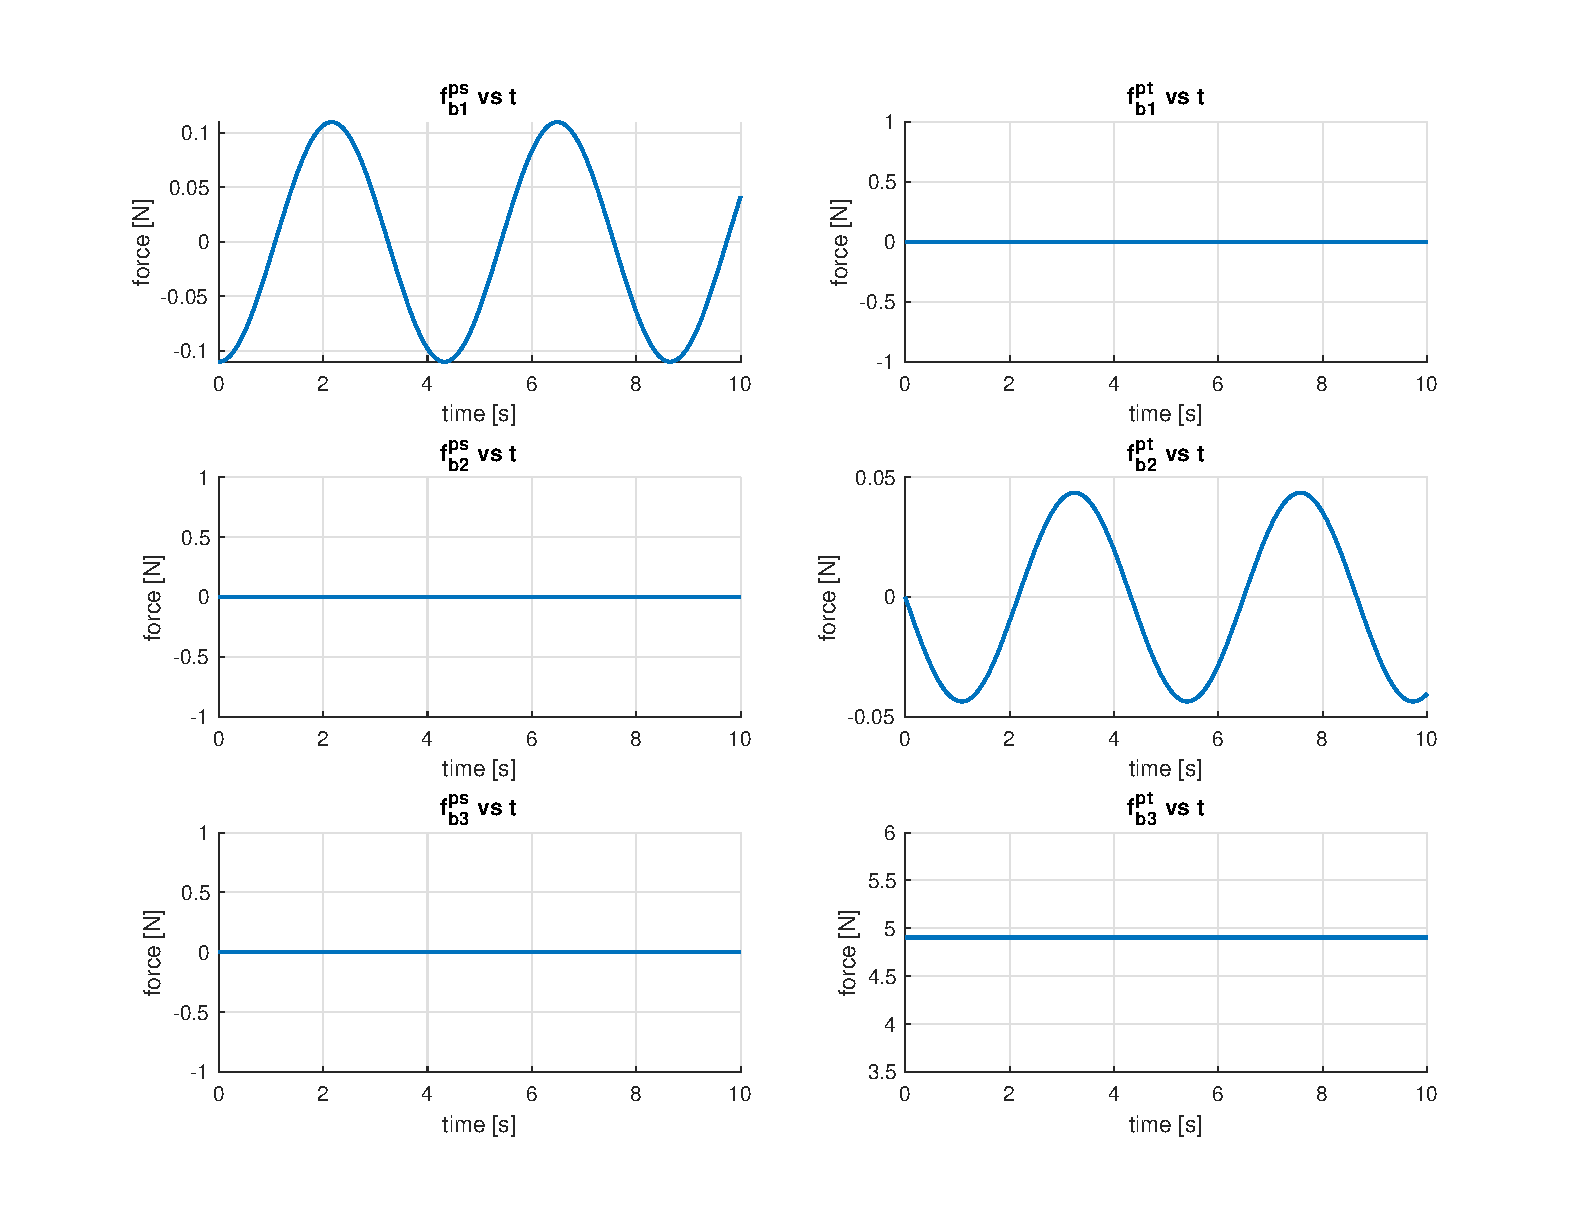
\includegraphics[width=1\textwidth]{P1c}
    \caption{$\mbf{f}_b^{pt}$ and $\mbf{f}_b^{ps}$ vs time.}
    \label{fig:P1c}
\end{figure}
\end{document}


